%% LaTeX Beamer presentation template (requires beamer package)
%% see http://latex-beamer.sourceforge.net/
%% idea contributed by H. Turgut Uyar
%% template based on a template by Till Tantau
%% this template is still evolving - it might differ in future releases!

%
% This document content was realized for the Marcusevans presentation
% on June 17th 2010
%
% Authors: ekeller
%


\documentclass{beamer}

\mode<presentation>
{
\usetheme{Warsaw}

\setbeamercovered{transparent}
}

\usepackage[english]{babel}
\usepackage[latin1]{inputenc}

% font definitions, try \usepackage{ae} instead of the following
% three lines if you don't like this look
\usepackage{mathptmx}
\usepackage[scaled=.90]{helvet}
\usepackage{courier}


\usepackage[T1]{fontenc}


\title[Continuous Integration]{Continuous Integration}

%\subtitle{at HAMILTON-Medical AG}

% - Use the \inst{?} command only if the authors have different
%   affiliation.
%\author{F.~Author\inst{1} \and S.~Another\inst{2}}
\author{Eric Keller}

% - Use the \inst command only if there are several affiliations.
% - Keep it simple, no one is interested in your street address.
\institute[HAMILTON-Medical AG]
{
HAMILTON-Medical AG\\
Platform C
}

\date{2010-06-17 / Industrialisierung Embedded Software Engineering}

% This is only inserted into the PDF information catalog. Can be left
% out.
\subject{Talks}



% If you have a file called "university-logo-filename.xxx", where xxx
% is a graphic format that can be processed by latex or pdflatex,
% resp., then you can add a logo as follows:

\pgfdeclareimage[height=0.5cm]{hamilton-logo}{../img/hamilton-logo.jpg}
\logo{\pgfuseimage{hamilton-logo}}


% Delete this, if you do not want the table of contents to pop up at
% the beginning of each subsection:
\AtBeginSubsection[]
{
\begin{frame}<beamer>
\frametitle{Outline}
\tableofcontents[currentsection,currentsubsection]
\end{frame}
}

% If you wish to uncover everything in a step-wise fashion, uncomment
% the following command:

%\beamerdefaultoverlayspecification{<+->}

\begin{document}

\begin{frame}
\titlepage
\end{frame}

% goal and policy
%\section*{Presentation goals and policy}
\begin{frame}
\frametitle{Goals and policy}
Goals:
\begin{itemize}
  \item Give an overview of what can be achieved with Continuous Integration
  (CI)
  \item Share knowledge and ideas
\end{itemize}

\begin{block}{Presentation policy}
   \alert{Please note your question and keep them warm for the end of the
   presentaion}
 \end{block}

% You might wish to add the option [pausesections]
\end{frame}



\begin{frame}
\frametitle{Outline}
\tableofcontents
% You might wish to add the option [pausesections]
\end{frame}

%% frame pattern
%\begin{frame}
%\frametitle{}
%\framesubtitle{Subtitles are optional}
%\end{frame}

\section{Introduction}

\subsection[About Hamilton-Medical]{About Hamilton-Medical}
\begin{frame}
\frametitle{Activities and organisation}
\begin{columns} 
  \column{.5\textwidth}
    \begin{block}{Platform C}
      \begin{center}
	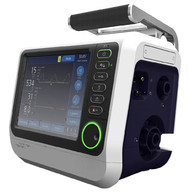
\includegraphics[height=2cm]{../img/C1.png}
	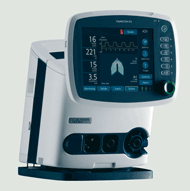
\includegraphics[height=2cm]{../img/C2.png}
      \end{center}
    \end{block}

    \begin{block}{Platform G}
      \begin{center}
	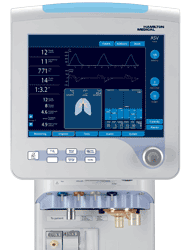
\includegraphics[height=2cm]{../img/G5.png}
      \end{center}
    \end{block}

  \column{.5\textwidth}
    \begin{block}{Accessories}
      \begin{center}
	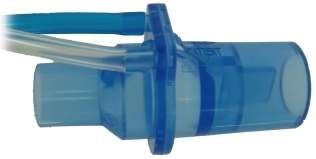
\includegraphics[height=2cm]{../img/flowsensor.png}
      \end{center}
    \end{block}
\end{columns}

\end{frame}

\subsection[Developer environment]{Developer environment}
\begin{frame}{Host development tools}
The Platform C Projects are developed on Microsoft Windows Host, using the
following software and hardware:
\begin{columns}
	\column{.5\textwidth}
	\begin{block}{Software Development}
	\begin{itemize}
		\item<1-> IBM Rational Rhapsody
  		\item<2-> WindRiver Workbench (eclipse) 
  		\item<3-> IPL Cantata++
    \end{itemize}
    \end{block}

	\begin{block}{Other used tools}
	\begin{itemize}
      \item<4-> shell, perl, scripting
      \item<5-> PVCS version manager
      \item<6-> ScrumWorks 
    \end{itemize}
    \end{block}

	\column{.5\textwidth}
	\begin{block}{Target Development}
	\begin{itemize}
      \item<7->WindRiver VxWorks 6.4
  	  \item<8-> Power PC MPC5200 B
    \end{itemize}
    \end{block}
\end{columns}
\end{frame}

%\section[Key notes]{Key notes}
\begin{frame}
\frametitle{Continuous integration key notes}
\begin{itemize}
  \item CI is a software development practice where software parts are
  integrated frequently
  \item Each integration step is verified by an automated process
  \item Find problems as soon as possible
  \item Make it easy for anyone to get the latest executable
  \item CI is all about communication
\end{itemize}
\end{frame}

\section[Automated build and test]{Automated build and test}
\subsection[Technical notes]{Technical notes}

\subsection[Good practices]{Good practices}

\subsection[Prerequisites]{Prerequisites}

\section[Automated deployment]{Automated deployment}

\subsection[Notifications and list of changes]{Notifications and list of
changes}

\subsection[Get the latest versions]{Get the latest versions}

\subsection[feedbacks]{Feedbacks}

\section[Benefits and optimisation]{Benefits and optimisation}


\section*{Summary}

\begin{frame}
\frametitle<presentation>{Summary}

\begin{itemize}
  \item The \alert{first main message} of your talk in one or two lines.
\end{itemize}

% The following outlook is optional.
\vskip0pt plus.5fill
\begin{itemize}
  \item Outlook
  \begin{itemize}
    \item Something you haven't solved.
    \item Something else you haven't solved.
  \end{itemize}
\end{itemize}
\end{frame}

\end{document}
